%
% Titelpagina
%

\maketitle


%
% Copyright
%

\null
\vfill

Copyright © 2011 Tim Besard

\vspace{1cm}

\begin{wrapfigure}{l}{2.5cm}
\vspace{-10pt}
\centering
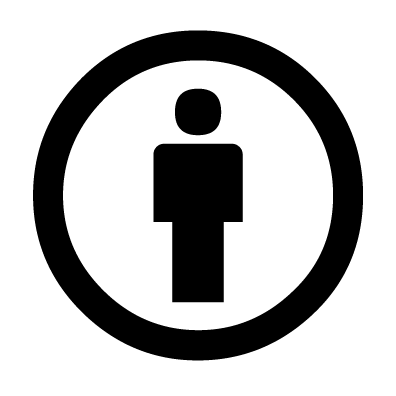
\includegraphics[width=2.5cm]{afbeeldingen/creative-commons-by}
\end{wrapfigure}

\noindent \nohyphens{Dit werk is gelicenseerd onder een Creative Commons Naamsvermelding 2.0 België licentie (\code{CC BY 2.0 BE}). Een kopie van deze licentie is te verkrijgen op de \makeurl{http://creativecommons.org/licenses/by/2.0/be/}{website van Creative Commons}, of door een brief te sturen naar \texttt{Creative Commons, 171 Second Street, Suite 300, San Francisco, California, 94105, USA}}.


%
% Abstract
%

\cleardoublepage

\selectlanguage{dutch}
\begin{abstract}
Het doel van deze thesis is de ontwikkeling van een modern multimediaframework ter vervanging van het verouderde systeem in de volkssterrenwacht MIRA. Het framework moet instaan voor de opslag, distributie, en weergave van multimediafragmenten, alsook de nodige middelen bieden zodat een designer er aantrekkelijke en veelzijdige presentaties kan voor ontwerpen.

Eerst en vooral wordt het systeem ingedeeld in de nodige deelsystemen, en hebben we na een grondige studie vastgelegd hoe die deelsystemen met elkaar communiceren. Zo zal de opslag en distributie gerealiseerd worden door een centrale server, die de kiosken zal detecteren en configureren via \acs{upnp}. Dataopslag en -overdracht zal gerealiseerd worden door gebruik te maken van een \acs{svn} repository, waarbij de presentaties opgemaakt zullen zijn in \acs{html} en Javascript.

Vervolgens worden alle deelsystemen geïmplementeerd. Waar we voor de server enkel voorzien in een Java-applicatie die alle vereiste taken uitvoert, zorgen we voor de kiosken naast de Qt-applicatie tevens voor de nodige hardware. Hiervoor selecteren we een gepaste embedded computer en stellen we een besturingssysteem samen die de applicatie adequaat kan uitvoeren. Ook voorzien we in een inputmodule die instaat voor het verwerken van gebruikersinvoer, waarvoor we een printplaat ontwerpen en zorgen voor de bijhorende firmware.
\end{abstract}

\clearpage

\selectlanguage{english}
\begin{abstract}
The purpose of this applied dissertation is to develop a modern multimedia framework replacing an outdated system in the astronomy museum MIRA. The framework has to take care of data storage, distribution, and visualisation. It should also offer the means for a designer to develop visually appealing and versatile presentations.

Before all else, we divide the system in several subcomponents, and determine the exact interface between them. In order to do this, we carefully select the best technologies to accomplish each task: storage and distribution shall be taken care of by a central server, discovering and configuring any clients using the \acs{upnp} protocol. To accomplish efficient storage and distribution, a \acs{svn} repository will be used. Finally, the presentations will be formatted using \acs{html} and Javascript.

Thereafter we proceed to the actual implementation of each subsystem. While the server-application will only consist of a single Java application, the clients need some more work. Not only do we create a Qt-based application to perform all necesary tasks, we also need to select the proper hardware to run that application on. This means selecting an appropriate embedded computer, and compiling an operation system capable of running our application. We also develop the \acs{pcb} and firmware for an input module to take care of any user input.
\end{abstract}

\selectlanguage{dutch}

\clearpage

%
% Voorwoord
%

\chapter*{Voorwoord}
\addcontentsline{toc}{chapter}{Voorwoord}

\textit{Hier komt het voorwoord.}

\clearpage


%
% Inhoudstafel
%

\setlength\cftpartnumwidth{2em}
\tableofcontents

\clearpage


%
% Lijst met afbeeldingen
%

\listoffigures

\clearpage


%
% Lijst met fragmenten
%

\renewcommand{\lstlistlistingname}{Lijst van fragmenten}
\renewcommand{\lstlistingname}{Fragment}
\markboth{List van fragmenten}{Lijst van fragmenten}
\addcontentsline{toc}{chapter}{Lijst van fragmenten}
\lstlistoflistings
% TODO: probleem als meer dan 1 pagina aan fragmenten

\clearpage


%
% Lijst van afkortingen
%

\chapter*{Lijst van afkortingen}
\markboth{List van afkortingen}{Lijst van afkortingen}
\addcontentsline{toc}{chapter}{Lijst van afkortingen}

\begin{acronym}[WYSIWYG]	% langste afkorting
\acro{agpl}[AGPL]{\acs{gnu} Affero General Public License}
\acro{ajax}[Ajax]{Asynchronous JavaScript and XML}
\acro{ajp}[AJP]{Apache JServ Protocol}
\acro{api}[API]{Application Programming Interface}
\acro{cc-by}[CC-BY]{\acl{cc} Attribution}
\acro{cc}[CC]{Creative Commons}
\acro{cc-sa}[CC-SA]{\acl{cc} ShareAlike}
\acro{corba}[CORBA]{Common Object Request Broker Architecture}
\acro{cpu}[CPU]{Central Processing Unit}
\acro{dcp}[DCP]{Device Control Protocol}
\acro{dhcp}[DHCP]{Dynamic Host Configuration Protocol}
\acro{dns}[DNS]{Domain Name System}
\acro{dru}[DRU]{Design Rules}
\acro{dsp}[DSP]{Digital Signal Processor}
\acro{eeprom}[EEPROM]{Electrically Erasable Programmable Read-Only Memory}
\acro{fpu}[FPU]{Floating-Point Unit}
\acro{fsf}[FSF]{Free Software Foundation}
\acro{gcc}[GCC]{\acs{gnu} compiler collection}
\acro{gnu}[GNU]{GNU's Not Unix!}
\acro{gpl}[GPL]{\acs{gnu} General Public License}
\acro{gpu}[GPU]{Graphics Processing Unit}
\acro{hid}[HID]{Human Interface Device}
\acro{html}[HTML]{Hypertext Markup Language}
\acro{http}[HTTP]{Hypertext Transport Protocol}
\acro{hvsp}[HVSP]{High-Voltage Serial Programming}
\acro{ip}[IP]{Internet Protocol}
\acro{isp}[ISP]{In-System Programming}
\acro{jar}[JAR]{Java ARchive}
\acro{jvm}[JVM]{Java Virtual Machine}
\acro{kde}[KDE]{K Desktop Environment}
\acro{lgpl}[LGPL]{\acs{gnu} Lesser General Public License}
\acro{lufa}[LUFA]{Lightweight USB Framework for AVRs}
\acro{mac}[MAC]{Media Access Control}
\acro{maven}[Maven]{Apache Maven}
\acro{mdns}[mDNS]{Multicast DNS}
\acro{mit}[MIT]{Massachusetts Institute of Technology}
\acro{moc}[MOC]{Meta-Object Compiler}
\acro{mpl}[MPL]{Mozilla Public License}
\acro{nas}[NAS]{Network Attached Storage}
\acro{ohl}[OHL]{Open Hardware License}
\acro{pcb}[PCB]{Printed Circuit Board}
\acro{pll}[PLL]{Phase-Locked Loop}
\acro{pom}[POM]{Project Object Model}
\acro{ram}[RAM]{Random Access Memory}
\acro{rest}[REST]{Representational State Transfer}
\acro{rhel}[RHEL]{Red Hat Enterprise Linux}
\acro{rmi}[RMI]{Remote Method Invocation}
\acro{rpc}[RPC]{Remote Procedure Call}
\acro{scpd}[SCPD]{Service Control Protocol Description}
\acro{sl}[SL]{Scientific Linux}
\acro{soap}[SOAP]{Simple Object Access Protocol}
\acro{ssdp}[SSDP]{Simple Service Discovery Protocol}
\acro{ssl}[SSL]{Secure Socket Layer}
\acro{svn}[SVN]{Apache Subversion}
\acro{uart}[UART]{Universal Asynchronous Receiver/Transmitter}
\acro{upnp}[UPnP]{Universal Plug and Play}
\acro{usb}[USB]{Universal Serial Bus}
\acro{uuid}[UUID]{Universally Unique Identifier}
\acro{webdav}[WebDAV]{Web-based Distributed Authoring and Versioning}
\acro{wtfpl}[WTFPL]{Do What The Fuck You Want Public License}
\acro{wysiwyg}[WYSIWYG]{What You See Is What You Get}
\acro{xml}[XML]{eXtensible Markup Language}
\acro{xsd}[XSD]{XML Schema Definition}
\end{acronym}

\acresetall
\clearpage
